\documentclass[12pt,a4paper]{article}
\usepackage[utf8]{inputenc}
\usepackage[IL2]{fontenc}
\usepackage{amsmath}
\usepackage{amsfonts}
\usepackage{amssymb}
\usepackage{graphicx}
\usepackage{xcolor}



%\title{Automatizovaná detekce a klasifikace jevů v časových řadách hydraulických sensorů}
\title{Automatized detection and classification of events in the time series of hydraulic sensors}
\author{Alexander Ma\v{c}ejovsk\'{y} \and \v{S}t\v{e}p\'{a}n Pardubick\'{y}}
\date{\today}

\begin{document}

%%\begin{titlepage}
%%    \centering
%%    \vspace*{2cm}
%%    {\huge\bfseries \maketitle}
%%    \vfill
   % \emph{Last edited on:} \today % Date will update automatically
%%    \vfill
%%\end{titlepage}

\maketitle % Insert title here

\thispagestyle{empty} % Remove page number from title page

\clearpage % Start the table of contents on a new page

\tableofcontents  


 

\newpage

\section{Introduction}
 
The domain of sewage man agement is critical for urban infrastructure, but it is also often overlooked.
The traditional methods of monitoring sewage systems are constrained by the limitations of manual analysis, often resulting in delayed responses to anomalies and missed opportunities for optimization.
\textcolor{green}{Are we capable of making such judgements (Im not)? Anyway, the task was given by the client, general importance is beside the point.}
Our goal was to create a Python library encapsulating a suite of algorithms, each meticulously designed to address data exploration, anomaly detection, visualization and correction of errors. Leveraging the power of Python's extensive ecosystem of libraries for scientific computing and data analysis, our solution easily integrates into existing workflows, offering a utility for both experts and practitioners in the field. This paper will summarize our work process and display our results to the reader.


\textcolor{green}{My version: DHI is a water management company. Its portfolio includes water canals and pipelines with both fresh and waste water. The company uses physical models for predicting amount of flow in different locations. The quality of these models needs to be verified by empirical data collected by sensors situated directly in the canals and pipes which measure water level and velocity. Such measurements are then used for calculation of the water flow. Unfortunately, the sensors are not flawless as they can get clogged or otherwise corrupted by various objects flowing in the water.   The fact a sensor reports faulty data can be usually detected by visual inspection of the resulting time series of its measurements. The goal of this project is to develop algorithms for automatized detection and, ideally, correction of such measurement errors.}



\begin{figure}[ht]
  \noindent\makebox[\textwidth]{%
  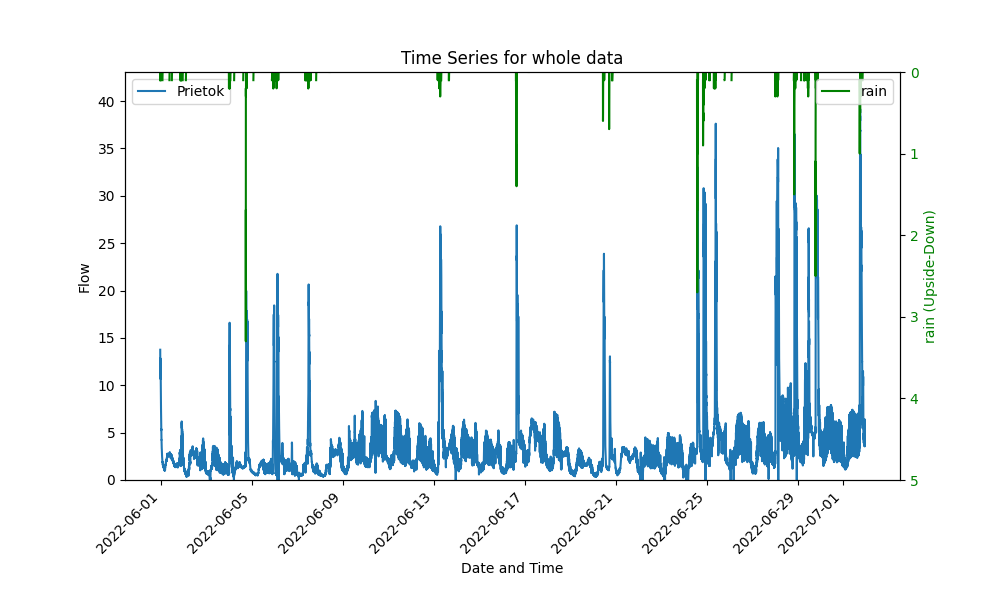
\includegraphics[width=1.4\textwidth]{Rain Dataset.png}}
  \caption{Example of a time series of flow in sewage pipe and measured precipitation. It can be seen that the peeks in the flow coincide with rain.}
    \label{rain_data}
\end{figure}

We were given several time series of flow of water in a sewage system. Each datapoint describes aggregated amount of water that has flown through a fixed control part of a sewer. This amount was calculated from the measured level of the water, it's velocity and the shape of the pipe. This information is gathered by means of various (often pricey) sensors. These sensors can be prone to various types of malfunctions. They can get clogged, displaced or even break. It is important to be able to detect these forms of failures in the time series. The time series of the flow is however very volatile and noisy. It features major upticks in flow coinciding with rain and natural daily cyclicity (peeks and increased volatility in the mornings and evenings when people tend to bathe and use toilet, dishwasher among other causes). Example can be seen in Figure \ref{rain_data}. These fluctuations make it hard to detect malfunctions.

\textcolor{green}{My version: We were given time series of the water level, velocity and flow from various measurement stations.  These time series are quite  volatile and noisy. They feature major upticks  coinciding with rain and natural daily cyclicity (peeks and increased volatility in the mornings and evenings when people tend to use shower, dishwasher etc.), see Figure \ref{rain_data} for an example.}

The client wanted us to try to come up with an original solution to the problem not influenced by their own currently implemented methods. As such we were given little to no information as to what the errors look like and how to correct them. Due to neither of us having any expertise in the field of sewage management, our work should be seen as an attempt to innovatively explore an unknown field and develop new solutions. As such, our approach was to creatively utilize standard techniques for working with time series and create a framework for their further utilization, rather than using or developing overly complex methods.


\subsection{Task Description}
Our main task is to develop a Python library for automatized detection and correction of  measurement errors in the time series of water velocity, level and flow. It can be broken down into the following steps:
\begin{itemize}
  \item Data exploration
  \item Handling of rain and cyclicity
  \item Definition and identification of errors
  \item Correction of errors
  \item Development of Python library for handling all of these steps
\end{itemize}

We were given several restrictions for how to proceed and what should our methods (not) use:
\begin{itemize}
    \item While the precipitation data is very useful for understanding involved time series, it cannot be accessed by the methods.
    \item Each time series should be viewed in isolation, data from different time series should not be directly used in the same process.
    \begin{itemize}
      \item{We should not fit a big model on all the data and then use it on individual series.}
      \item{We cannot utilize any relations between the series (for example to investigate several series in parallel).}
      \end{itemize}
      \item {We are not given any target data, that is labels for errors or non-defunct (corrected) series for testing the performance.}
      \item{While information for both water level and velocity is provided, the time series are to be investigated as univariate - the methods should be developed for the flow and then can be later tried on other variables.}
      \item {If possible, need for utilizing methods in the real-time or with the minimal delay should be considered. }
    
%Note that the lack of any labels is very prohibitive...
\end{itemize}


We managed to identify three broad types of apparent errors occurring in the data and propose their corrections depending on how long the respective sensor malfunction lasts. The actual implementation of the corrections has been in some cases  due to time limitations only partially accomplished. The following sections describe in greater detail the data we obtained for the task, the identification of potential errors, their corrections, further ideas and suggestions for future development, and brief description of the resulting Python library. 


\newpage
\section{Data Exploration}
In this section we will focus on exploration and description of the data. We were provided with 43 csv files. After carefully examining them and extracting their contents we are able to gather information about 8 different measuring sessions. These sessions span approximately 30-110 days and the entries come in two minute intervals. Each session thus contains approximately 22000 - 80000 individual data points. The extracted variables of interests are:\footnote{Note that we do not include the units in which the individual measurements come. This information was not shared with us by the client and cannot be easily deduced (the units seem to vary among individual time series).}
\begin{itemize}
    \item Time
    \item Water level - measured by sensors
    \item Water velocity - measured by sensors
    \item Water flow - computed form water level, velocity and a known shape of the sewage pipe
    \item Precipitation - measured by sensors, only contained in one (smallest) measuring session
\end{itemize}


\textcolor{red}{TBD: Provide some explanatory statistics and suitable plots}




\newpage
\section{Identified Events}

\textcolor{red}{TBD: Describe identified events (errors), discuss them, show suitable plots}
\textcolor{green}{eventually done by visual inspection of series, other methods tried but found inadequate given time limitations and lack of targets (see section on other ideas),  identification based on heuristic rules seems to work acceptably well}\\

\textcolor{green}{TO DO: describe used notation}

\textcolor{green}{perhaps TO DO: add mathematical formalization of the task}

\subsection{Constant and Zero Values}
\textcolor{green}{from presentations}

Zero values are simply those for which $v_t = 0$. We identify constant observations as those which have not changed in comparison to past and future, i.e. observation at $t$ is constant if $v_{t-1} = v_t = v_{t+1}$. Technically, this is done by identifying zero moving standard deviation of the flow  with window 3,
$$ Msd_t(W_0) = 0 $$
with $W_0 = 3$. However, we recognize constant values only if there is at least $tol\_const = 5$ of them in succession, otherwise they are ignored as regular observations. Generally, we can be also more lenient by setting $W_0$ to some higher value.

\textbf{data requirements}: immediate identification of zero values and delay of only 1 period for constant values.

\subsection{Heightened Volatility}
Sometimes, flow is suspiciously volatile. We identify this by high values of its (or rather of its first differences') moving standard deviation,
$$ Msd_t(W_2) > K $$
where we chose window $W_2 = 30$. Threshold is determined as overall standard deviation for lower 0.7 quantile of flow observations (rough controlling for rain disturbances),
$$ K = c_2 \cdot \sigma_{p_1} $$
with $c_2 = 1$ and $p_1 = 0.7$, $\sigma_{p_1} = sd(v_t; v_t \leq p_1\text{th quantile of the (first diffs. of the) flow})$. These are default values, choosing lower $p_1$ or $c_2$ would be more sensitive to heightened volatility and vice versa.

We furthemore identify groups of high volatility observations (successive periods in which high volatility is recognized) and if there are two groups seperated by less then $tol\_vol_1 = 5$ non-volatile observations we merge them by setting observations between them as high-volatility observations as well. On the other hand if a group of highly volatile observations has less then $tol\_vol_2 = 5$ members we deem it as a false signal and categorize them as OK.

\textbf{data requirements}: We need $W_2$ observations for moving standard deviation calculations, i.e. \textbf{delay of 15 periods} at default setting. But we also need to have set the threshold $K$ for which we use the whole history of the data. If necessary could be set expertly to some reasonable value.


When it is raining it is natural and OK that volatility is high. We thus try to recognize when this happens due to rain. Rain is usually accompanied by heightened level of the flow (here, we always use flow, not its first differences), hence we set conditions for this category as
$$ \text{heightened volatility and }  MA_t(W_3) \geq p_2\text{th percentile of the flow.} $$
As default we set $p_2 = 0.9$ and $W_3 = 5$.

We furthermore perform the same kind of grouping as for general high volatility, this time with $tol\_rain_1 = 5$ and $tol\_rain_2 = 10$.

\textbf{data requirements}: This category is subset of heightened volatility, so \textbf{same as above}. Additionally, we need moving average with window $W_3$ but this window is in default setting smaller than the one required for heightened volatility identification. We use the whole history of the data for calculating $p_2$th percentile of the flow but if necessary, this  could be replaced by some expertly chosen value.


\subsection{Outliers}
Flow values which seems odd compared to nearby past and future values. $v_t$ is identified as outlier if flow jumped by high margin up and then immediately fell by high margin down (or vice versa, fell and than rised back), i.e.
$$ \Delta v_t > T_t \qquad \text{and} \qquad \Delta v_{t+1} < -T_t $$
or both inequalities in the opposite direction.

Threshold is based on moving standard deviation \textbf{of the first differences of the flow } as 
$$ T_t = c_1 \cdot Msd_t(W_1). $$
We use as default values $c_1 = 2.5$ and window $W_1 = 30$.

\textbf{data requirements }: for Msd we need $W_1$ observations, that is we can identify outliers with 15 periods = \textbf{ 30 minutes delay} with the default choice of $W_1$ but should probably work well with smaller windows, too.



\textcolor{green}{TO DO: add description of prolonged outliers, add logic and use of groupings, rewrite descriptions, add plots with examples, add table with percentages of identified events across main variables and sites,  add table with the default parameter values}







\newpage
\section{Corrections of Errors}

\textcolor{red}{TBD:Describe how and why we corrected the errors, why we kept some (volatility), provide suitable plots}

\newpage
\section{Performance Evaluation}
\textcolor{red}{TBD:no target $\Rightarrow$ not clear how to do this, but detection of events done expertly with the help of consultations,  basic idea for evaluation of corrections could be that no (only few) errors should be detected in already corrected time series }

\newpage
\section{Other Suggestions and Ideas}
\textcolor{red}{TBD: Describe some aproaches we tried, which didn't end up in final methods (More various methods of smoothing, Clustering, Autoencoder, describe why some unsupervised approaches failed (rain). Discuss posibility of future feature engineering approaches (this would require expert consultations and more collaboration from client}


\newpage
\section{Python Library}
\textcolor{red}{TBD:brief summary of what the resulting library contains, how it is used, + link to the github page (we should probably restrict it with a password)}


\newpage
\section{Utilized Python libraries}

In this section we give a quick summary of the most important Python libraries we used in the task an how we utilized them.

\subsection{NumPy \cite{harris2020array}}
NumPy, short for Numerical Python, is numerical computing library for Python. It is a fundamental library for scientific computing in Python and provides support for large, multi-dimensional arrays, along with a set of functions to operate on these efficiently. 

\textcolor{red}{TBD:Describe how we used it.}

\subsection{Pandas \cite{reback2020pandas}}

Pandas is a data manipulation and analysis library for the Python. It provides ability to efficiently manipulate large datasets. Pandas is built on top of the NumPy library.

\textcolor{red}{TBD:Describe how we used it.}



\subsection{Matplotlib \cite{Hunter:2007}}
Matplotlib is a data visualization library for the Python. It provides a wide variety of tools for creating high-quality charts, graphs, and figures. Matplotlib is designed to produce publication-quality visuals and is widely used in the fields of data science, machine learning, and scientific research.

\textcolor{red}{TBD:Describe how we used it.}

\subsection{Statsmodels \cite{seabold2010statsmodels}}

Statsmodels is a Python library for estimating and testing statistical models. It provides a wide set of tools for statistical analysis and hypothesis testing. Statsmodels includes functionalities for linear and non-linear regression models, time-series analysis and statistical testing.

\textcolor{red}{TBD:Describe how we used it.}

\subsection{Scikit-learn \cite{pedregosa2011scikit}}

Scikit-learn, often abbreviated as sklearn, is a Python machine learning library. It is built on top of other Python libraries such as NumPy, SciPy, and Matplotlib. Scikit-learn provides simple and efficient tools for feature engineering and development of AI models, making it a widely used library in the fields of machine learning and data science.

\textcolor{red}{TBD:Describe how we used it.}




\newpage
\section{Conclusion}
\textcolor{red}{TBD: Provide a conclusion, discuss what we acomplished, }

\clearpage
\bibliographystyle{unsrt}
\bibliography{references}


\end{document}